% Chương 1

\chapter{Xử lý ngôn ngữ tự nhiên - Natural language proccessing} % Tên của chương

\label{Chapter1} % Để trích dẫn chương này ở chỗ nào đó trong bài, hãy sử dụng lệnh \ref{Chapter1} 

%----------------------------------------------------------------------------------------

% Định nghĩa một số lệnh cần thiết để điều chỉnh định dạng cho một số nội dung nhất định trong bài
\newcommand{\keyword}[1]{\textbf{#1}}
\newcommand{\tabhead}[1]{\textbf{#1}}
\newcommand{\code}[1]{\texttt{#1}}
\newcommand{\file}[1]{\texttt{\bfseries#1}}
\newcommand{\option}[1]{\texttt{\itshape#1}}

%----------------------------------------------------------------------------------------

\section{Giới thiệu về xử lí ngôn ngữ tự nhiên (NLP)}

Xử lý ngôn ngữ tự nhiên là một nhánh của Trí tuệ nhân tạo, tập trung vào việc nghiên cứu sự tương tác giữa máy tính và ngôn ngữ tự nhiên của con người, dưới dạng tiếng nói (speech) hoặc văn bản (text)\cite{WEBSITE:1}.

Mục tiêu của lĩnh vực này là giúp máy tính hiểu và thực hiện hiệu quả những nhiệm vụ liên quan đến ngôn ngữ của con người như: tương tác giữa người và máy, cải thiện hiệu quả giao tiếp giữa con người với con người, hoặc đơn giản là nâng cao hiệu quả xử lý văn bản và lời nói.



%----------------------------------------------------------------------------------------

\section{Lịch sử hình thành và phát triển của NLP}

Xử lý ngôn ngữ tự nhiên ra đời từ những năm 40 của thế kỷ 20, trải qua các giai đoạn phát triển với nhiều phương pháp và mô hình xử lý khác nhau. Có thể kể tới các phương pháp sử dụng ô-tô-mát và mô hình xác suất (những năm 50), các phương pháp dựa trên ký hiệu, các phương pháp ngẫu nhiên (những năm 70), các phương pháp sử dụng học máy truyền thống (những năm đầu thế kỷ 21), và đặc biệt là sự bùng nổ của học sâu trong thập kỷ vừa qua\cite{WEBSITE:1}.

Xử lý ngôn ngữ tự nhiên có thể được chia ra thành hai nhánh lớn, không hoàn toàn độc lập, bao gồm xử lý tiếng nói (speech processing) và xử lý văn bản (text processing).

Xử lý tiếng nói tập trung nghiên cứu, phát triển các thuật toán, chương trình máy tính xử lý ngôn ngữ của con người ở dạng tiếng nói (dữ liệu âm thanh). Các ứng dụng quan trọng của xử lý tiếng nói bao gồm nhận dạng tiếng nói và tổng hợp tiếng nói.

Xử lý văn bản tập trung vào phân tích dữ liệu văn bản. Các ứng dụng quan trọng của xử lý văn bản bao gồm tìm kiếm và truy xuất thông tin, dịch máy, tóm tắt văn bản tự động, hay kiểm lỗi chính tả tự động. Xử lý văn bản đôi khi được chia tiếp thành hai nhánh nhỏ hơn bao gồm hiểu văn bản và sinh văn bản. Nếu như hiểu liên quan tới các bài toán phân tích văn bản thì sinh liên quan tới nhiệm vụ tạo ra văn bản mới như trong các ứng dụng về dịch máy hoặc tóm tắt văn bản tự động.

\section{Giao tiếp giữa người và máy dựa trên NLP}
Ngày nay, nhiều hệ thống/chương trình máy tính có khả năng giao tiếp với con người thông qua ngôn ngữ tự nhiên, hoặc dưới dạng văn bản, hoặc dưới dạng tiếng nói. Các ứng dụng tiêu biểu giao tiếp dưới dạng văn bản có thể kể đến như tìm kiếm thông tin, chatbot, dịch máy. Các ứng dụng giao tiếp qua tiếng nói như trợ lý ảo, tìm kiếm bằng giọng nói (điện thoại, tivi), và điều khiển qua giọng nói (điện thoại, các thiết bị gia đình)\cite{WEBSITE:1}.

Hình \ref{pic1.1} mô tả kiến trúc tiêu biểu của một chương trình máy tính giao tiếp với con người qua tiếng nói. Chương trình sẽ bao gồm các bước cơ bản sau:
\begin{figure}[h!]
	\centering
	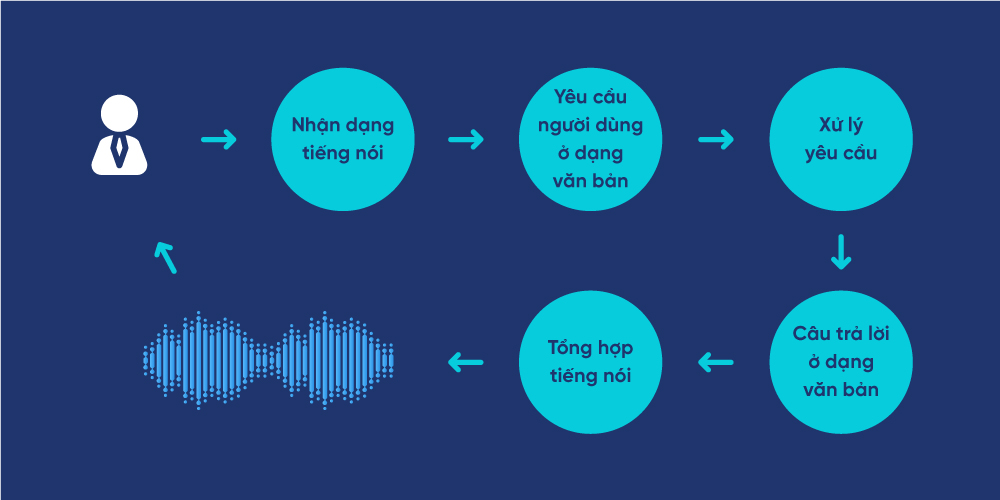
\includegraphics[width=1\textwidth]{
		nlp.jpg
	}
	\caption[Kiến trúc của một chương trình máy tính giao tiếp với con người thông qua tiếng nói ]{
		Kiến trúc của một chương trình máy tính giao tiếp với con người thông qua tiếng nói \label{pic1.1}
	}
\end{figure}


\begin{itemize}
	\item  Nhận dạng tiếng nói: ở bước này, máy tính sẽ nhận dạng yêu cầu của người dùng ở dạng tiếng nói và chuyển yêu cầu này về dạng văn bản.
	\item Xử lý yêu cầu: máy tính sẽ phân tích yêu cầu ở dạng văn bản, xử lý, đưa ra câu trả lời sử dụng các kỹ thuật trong xử lý văn bản.
	\item Tổng hợp tiếng nói: ở bước này, câu trả lời sẽ được chuyển từ dạng văn bản sang tiếng nói và gửi tới người dùng.
\end{itemize}


\section{Các bài toán cơ bản trong NLP } 
---------------------------------
\subsection{Mô hình hóa ngôn ngữ (Language modelling)}
Mô hình hóa ngôn ngữ (LM) gán một xác suất cho bất kỳ chuỗi từ nào. Về cơ bản, trongbài toán này, ta cần dự đoán từ tiếp theo xuất hiện theo trình tự, dựa trên lịch sử của các từ đã xuất hiện trước đó. LM rất quan trọng trong các ứng dụng khác nhau của NLP, và là lý do tại sao máy móc có thể hiểu được thông tin định tính. Một số ứng dụng của Mô hình hóa ngôn ngữ bao gồm: nhận dạng giọng nói, nhận dạng ký tự quang học, nhận dạng chữ viết tay, dịch máy và sửa lỗi chính tả.\cite{WEBSITE:3}

\subsection{Phân loại văn bản (Text classification)}
Phân loại văn bản gán các danh mục được xác định trước cho văn bản dựa trên nội dung của nó. Cho đến nay, phân loại văn bản là ứng dụng phổ biến nhất của NLP, được sử dụng để xây dựng các công cụ khác nhau như trình phát hiện thư rác và chương trình phân tích cảm xúc.\cite{WEBSITE:3}

\subsection{Trích xuất thông tin (Information extraction)}
Trích xuất thông tin (IE) tự động trích xuất thông tin có liên quan từ các tài liệu văn bản không có cấu trúc và / hoặc bán cấu trúc. Ví dụ về các loại tài liệu này bao gồm lịch sự kiện từ email hoặc tên của những người được đề cập trong một bài đăng trên mạng xã hội.\cite{WEBSITE:3}

\subsection{Truy xuất thông tin (Information retrieval)}
Google là một loại hệ thống Truy xuất Thông tin (IR) phổ biến nhất mà chúng ta thường sử dụng. IR làm nhiệm vụ tìm kiếm các tài liệu có liên quan từ một bộ dữ liệu lớn các tài liệu liên quan đến truy vấn do người dùng thực hiện.\cite{WEBSITE:3}

\subsection{Tác tử phần mềm hội thoại (Conversational agent)}
Tác tử phần mềm hội thoại thuộc AI hội thoại, liên quan đến việc xây dựng các hệ thống đối thoại mô phỏng các tương tác của con người. Các ví dụ phổ biến về AI hội thoại bao gồm Alexa, Siri, Google Home, Cortana, hay trợ lý ảo ViVi. Các công nghệ như chatbot cũng được hỗ trợ bởi  tác tử phần mềm hội thoại và ngày càng phổ biến trong các doanh nghiệp.\cite{WEBSITE:3}

\subsection{Tóm tắt văn bản (Text summarization)}
Tự động tóm tắt là quá trình rút ngắn một tập hợp dữ liệu để tạo một tập hợp con đại diện cho thông tin quan trọng nhất hoặc có liên quan trong nội dung gốc.\cite{WEBSITE:3}

\subsection{Hỏi đáp (Question answering)}
Hỏi đáp là bài toán xây dựng các hệ thống có thể tự động trả lời cho các câu hỏi do con người đặt ra bằng ngôn ngữ tự nhiên.\cite{WEBSITE:3}

\subsection{Dịch máy (Machine translation)}
Dịch máy (MT) là một nhánh con của ngôn ngữ học tính toán liên quan đến việc chuyển đổi một đoạn văn bản từ ngôn ngữ này sang ngôn ngữ khác. Một ứng dụng phổ biến của loại này là Google Dịch.\cite{WEBSITE:3}

\subsection{Mô hình hóa chủ đề (Topic modelling)}
Mô hình hóa chủ đề là một kỹ thuật Học máy không giám sát giúp khám phá cấu trúc chủ đề của một bộ tài liệu lớn. Ứng dụng NLP này là một công cụ khá phổ biến, được sử dụng trên nhiều lĩnh vực khác nhau – như Văn học, và Tin sinh học.\cite{WEBSITE:3}


%----------------------------------------------------------------------------------------

\section{Các công cụ giải quyết các bài toán NLP} 
\subsection{NLTK}
Natural Language ToolKit (NLTK) là một trong những nền tảng hàng đầu để xây dựng các chương trình Python xử lý và phân tích dữ liệu ngôn ngữ của con người. 

NLTK cung cấp giao diện dễ sử dụng cho hơn 50 tài nguyên ngữ liệu và từ vựng như mạng từ, cùng với một bộ thư viện xử lý văn bản để phân loại, mã hóa, tạo gốc, gắn thẻ, phân tích cú pháp và lập luận ngữ nghĩa.\cite{WEBSITE:3}

Ví dụ về sử dụng NLTK để xử lí dữ liệu

\lstinputlisting[style=codePython]{"Code/nltk.py"}

Kết quả:

\lstinputlisting[style=plaintext]{"Code/nltk_result.txt"}

\subsection{Spacy}
Bản phát hành đầu tiên của SpaCy là vào tháng 2 năm 2015, khiến nó trở thành một trong những framework nguồn mở gần đây dành cho các ứng dụng Xử lý ngôn ngữ tự nhiên Python. So với NLTK được tạo ra vào năm 2001, những người sáng tạo SpaCy có đủ thời gian để tìm hiểu NLTK và xem nó còn thiếu ở đâu. Một trong những cải tiến dễ nhận biết nhất so với NTLK bao gồm các cải tiến về hiệu suất, vì SpaCy sử dụng một số thuật toán mới nhất và tốt nhất.

Ngoài ra, SpaCy được ghi chép rất đầy đủ và được thiết kế để hỗ trợ khối lượng lớn dữ liệu. Nó cũng bao gồm một loạt các mô hình Xử lý ngôn ngữ tự nhiên được đào tạo trước, giúp việc học, giảng dạy và thực hành Xử lý ngôn ngữ tự nhiên với SpaCy trở nên dễ tiếp cận hơn \cite{WEBSITE:3}. 

Ví dụ tách chuỗi bằng spacy:

\lstinputlisting[style=codePython]{"Code/spacy.py"}

Ví dụ đọc dữ liệu từ file sau đó xử lí:

\lstinputlisting[style=codePython]{"Code/spacy1.py"}

Kết quả: 

\lstinputlisting[style=plaintext]{"Code/spacy_result.txt"}

\subsection{Stanford CoreNLP}
CoreNLP là một thư viện cực kỳ phổ biến cho các tác vụ Xử lý Ngôn ngữ tự nhiên, được xây dựng bởi cộng đồng NLP Stanford. Ngược lại với NLTK và SpaCy, được viết bằng Python hoặc Cython tương ứng, CoreNLP bằng Java – có nghĩa là máy tính của bạn sẽ cần phải có JDK (nhưng nó có API cho hầu hết các ngôn ngữ lập trình).

Trên trang chủ CoreNLP, các nhà phát triển mô tả CoreNLP là “nơi duy nhất để xử lý ngôn ngữ tự nhiên trong Java! CoreNLP cho phép người dùng lấy các chú thích ngôn ngữ cho văn bản, bao gồm mã thông báo và ranh giới câu, các phần của giọng nói, các thực thể được đặt tên, giá trị số và thời gian, trình phân tích cú pháp phụ thuộc và ý kiến chính, tình cảm, phân bổ trích dẫn và quan hệ. CoreNLP hiện hỗ trợ 6 ngôn ngữ: Ả Rập, Trung Quốc, Anh, Pháp, Đức và Tây Ban Nha.

Một trong những ưu điểm chính của CoreNLP là nó có khả năng mở rộng rất cao, trở thành lựa chọn phù hợp cho các tác vụ phức tạp. Một yếu tố khác là CoreNLP được xây dựng chú trọng đến tốc độ – nó được tối ưu hóa để vận hành cực kỳ nhanh. \cite{WEBSITE:3}

Ví dụ sử dụng Standford CoreNlp:

\lstinputlisting[style=codePython]{"Code/StandfordNLP.py"}

Kết quả:

\lstinputlisting[style=plaintext]{"Code/coreNLP-result.txt"}

\subsection{Gensim}
Gensim là một framework Python mã nguồn mở chuyên dụng, được sử dụng để biểu diễn tài liệu dưới dạng vectơ ngữ nghĩa theo những cách hiệu quả nhất và dễ dàng nhất có thể. Các tác giả đã thiết kế Gensim để xử lý văn bản thô, không có cấu trúc bằng cách sử dụng nhiều thuật toán học máy – vì vậy sử dụng Gensim để tiếp cận các tác vụ như Lập mô hình chủ đề là một ý tưởng tốt. Thêm vào đó, Gensim làm rất tốt việc xác định các điểm tương đồng trong văn bản, lập chỉ mục văn bản và điều hướng các tài liệu khác nhau.\cite{WEBSITE:3}

Gensim được xây dựng vì 3 lý do:

\begin{itemize}
	\item Tính thực tiễn – tập trung vào các thuật toán đã được chứng minh, đã được kiểm chứng để giải quyết các vấn đề thực tế của ngành. Gensim tập trung nhiều hơn vào kỹ thuật, ít hơn về học thuật.
	\item Độc lập đối với bộ nhớ – không cần toàn bộ kho dữ liệu đào tạo phải nằm hoàn toàn trong RAM cùng một lúc. Nó có thể xử lý kho dữ liệu lớn, quy mô web bằng cách sử dụng luồng dữ liệu.
	\item Hiệu suất – triển khai tối ưu hóa cao các thuật toán không gian vectơ phổ biến sử dụng C, BLAS và ánh xạ bộ nhớ
\end{itemize}

Ví dụ sử dụng Gensim:

\lstinputlisting[style=codePython]{"Code/gensim.py"}

Kết quả:

\lstinputlisting[style=plaintext]{"Code/gensim-result.txt"}
%----------------------------------------------------------------------------------------



			
			
			
